\chapter{Security Testing}

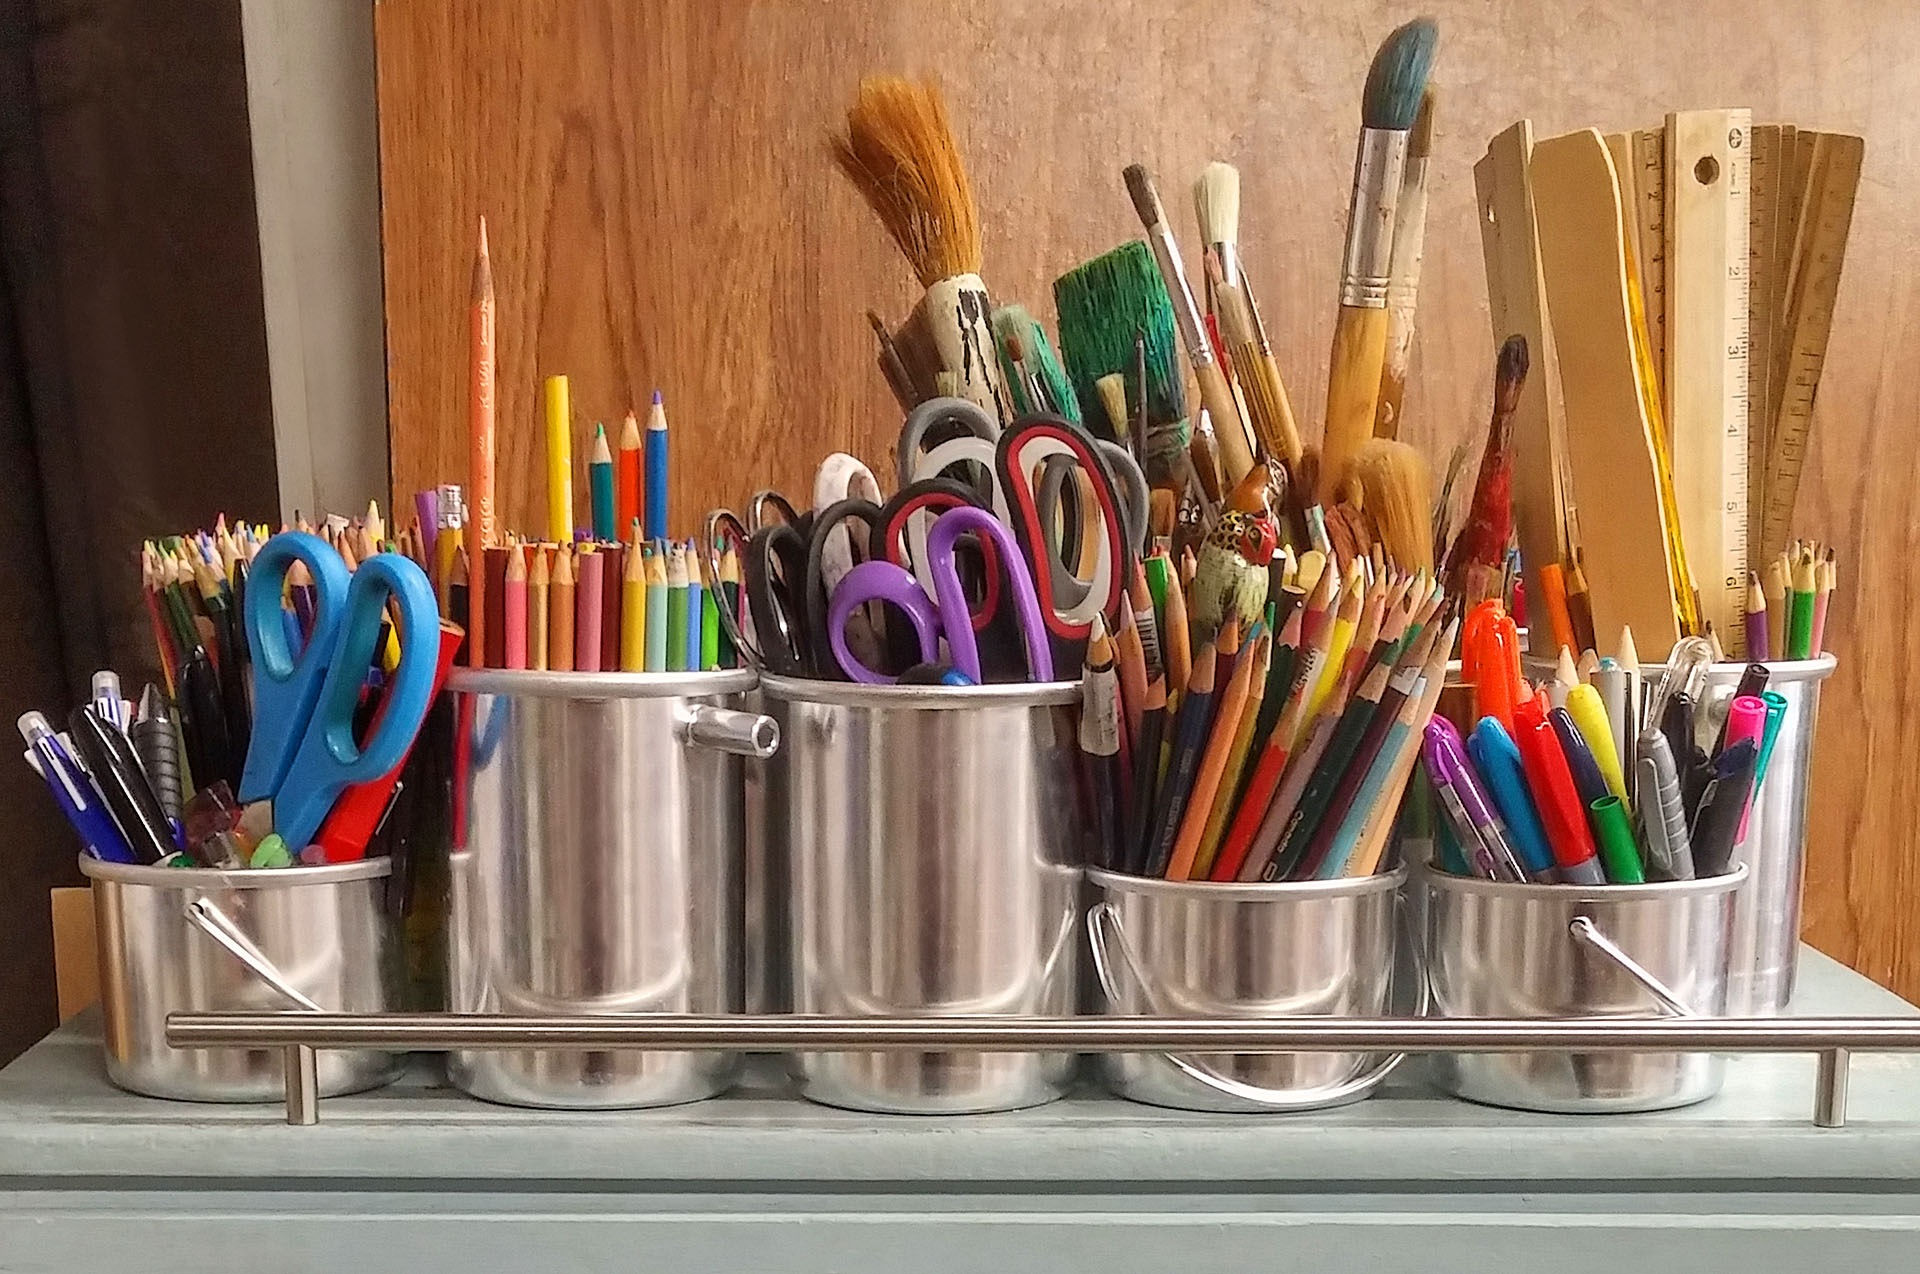
\includegraphics{31-security-testing.jpg}

This section is about things we can do to ensure we are driving out bugs and finding security issues as soon as possible in our product life cycle.

\markdownInput{../labs/31-security-testing/lab-31a-sec-test-setup.md}

\section{Code Scanning}

\markdownInput{../labs/31-security-testing/lab-31b-python-scanning.md}

\section{Validating Container Images}

\justifying
Lab with Hadolint and Trivy.

\markdownInput{../labs/31-security-testing/lab-31c-containers.md}

% lab - validating dependencies with ``safety''

\section{Directory Structure for Security Testing}

\justifying
Relevant files and folders related to our security testing framework are organized as seen below.

\begin{figure}[!htb]
    
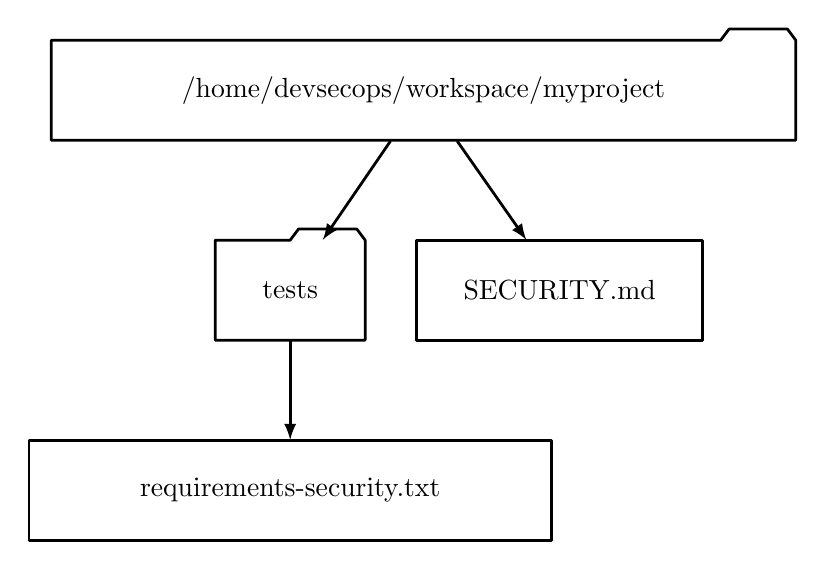
\begin{tikzpicture}[>=latex,line join=bevel,]
  \pgfsetlinewidth{1bp}
%%
\pgfsetcolor{black}
  % Edge: devsecops -> tests
  \draw [->] (130.13bp,143.7bp) .. controls (124.5bp,135.47bp) and (117.65bp,125.48bp)  .. (105.73bp,108.1bp);
  % Edge: devsecops -> md
  \draw [->] (154.11bp,143.7bp) .. controls (159.87bp,135.47bp) and (166.86bp,125.48bp)  .. (179.03bp,108.1bp);
  % Edge: tests -> req
  \draw [->] (94.0bp,71.697bp) .. controls (94.0bp,63.983bp) and (94.0bp,54.712bp)  .. (94.0bp,36.104bp);
  % Node: devsecops
\begin{scope}
  \definecolor{strokecol}{rgb}{0.0,0.0,0.0};
  \pgfsetstrokecolor{strokecol}
  \draw (276.0bp,180.0bp) -- (273.0bp,184.0bp) -- (252.0bp,184.0bp) -- (249.0bp,180.0bp) -- (8.0bp,180.0bp) -- (8.0bp,144.0bp) -- (276.0bp,144.0bp) -- cycle;
  \draw (142.0bp,162.0bp) node {/home/devsecops/workspace/myproject};
\end{scope}
  % Node: tests
\begin{scope}
  \definecolor{strokecol}{rgb}{0.0,0.0,0.0};
  \pgfsetstrokecolor{strokecol}
  \draw (121.0bp,108.0bp) -- (118.0bp,112.0bp) -- (97.0bp,112.0bp) -- (94.0bp,108.0bp) -- (67.0bp,108.0bp) -- (67.0bp,72.0bp) -- (121.0bp,72.0bp) -- cycle;
  \draw (94.0bp,90.0bp) node {tests};
\end{scope}
  % Node: md
\begin{scope}
  \definecolor{strokecol}{rgb}{0.0,0.0,0.0};
  \pgfsetstrokecolor{strokecol}
  \draw (242.5bp,108.0bp) -- (139.5bp,108.0bp) -- (139.5bp,72.0bp) -- (242.5bp,72.0bp) -- cycle;
  \draw (191.0bp,90.0bp) node {SECURITY.md};
\end{scope}
  % Node: req
\begin{scope}
  \definecolor{strokecol}{rgb}{0.0,0.0,0.0};
  \pgfsetstrokecolor{strokecol}
  \draw (188.0bp,36.0bp) -- (0.0bp,36.0bp) -- (0.0bp,0.0bp) -- (188.0bp,0.0bp) -- cycle;
  \draw (94.0bp,18.0bp) node {requirements-security.txt};
\end{scope}
%
\end{tikzpicture}


    \caption{Security testing related files.}
    \label{sectest}
\end{figure}
